\documentclass[a4paper,12pt]{article}
\usepackage{float}
\usepackage{pgfplots}
% Preamble: \pgfplotsset{width=1cm,compat=newest}
\begin{document}
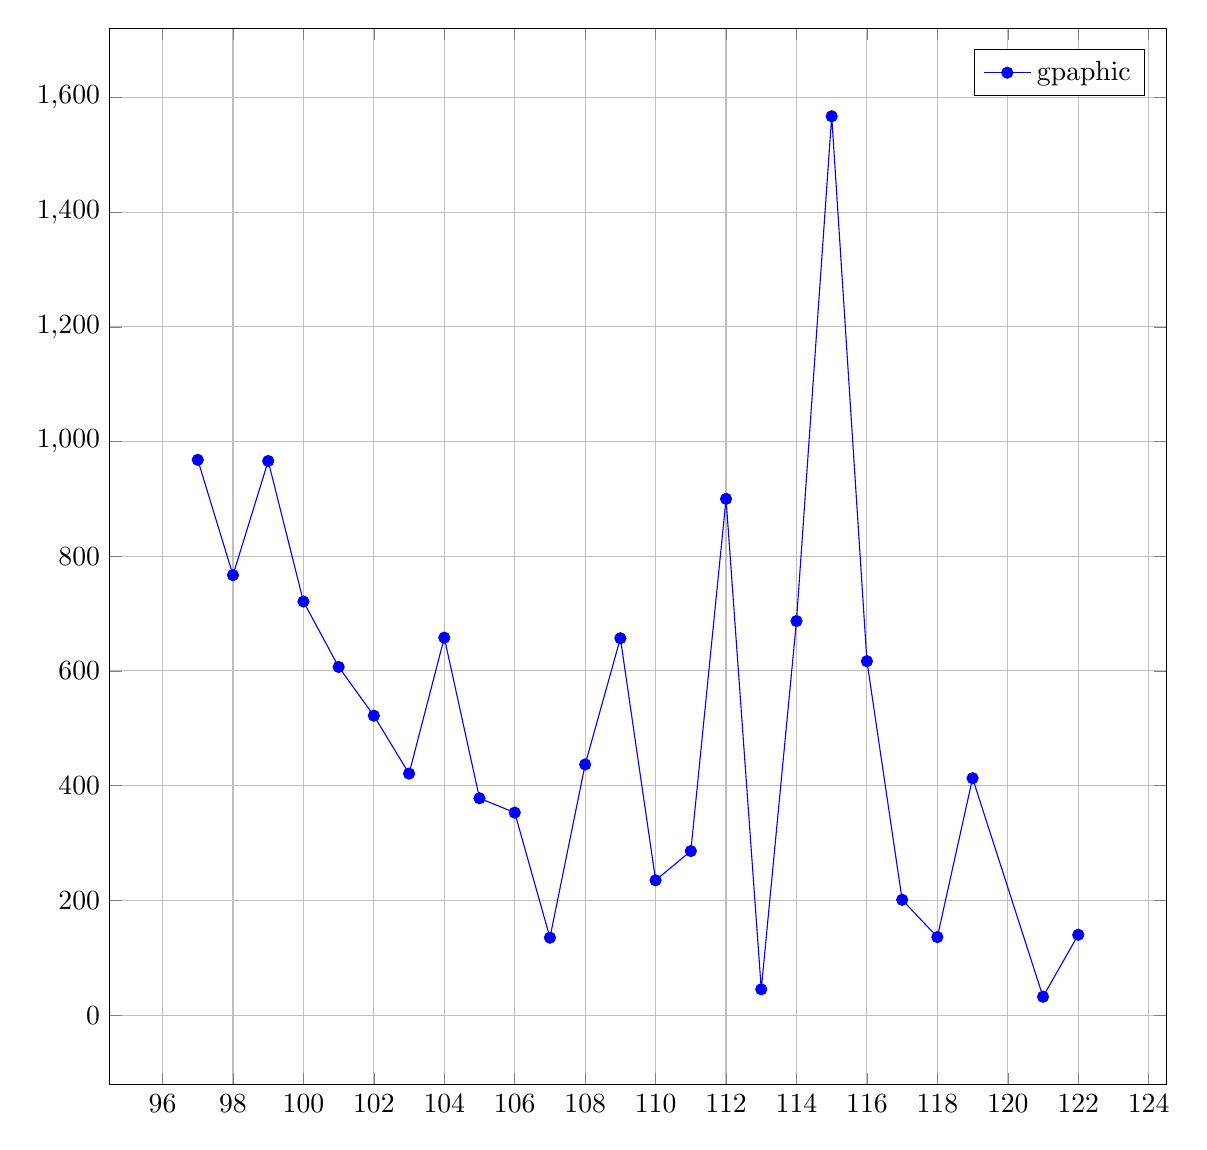
\begin{tikzpicture}
\begin{axis}[height=15cm,width=15cm,grid=major]
\addlegendentry{gpaphic}
\addplot[color = blue, mark = * ] coordinates {
(97,968)
(98,767)
(99,966)
(100,721)
(101,607)
(102,522)
(103,421)
(104,658)
(105,378)
(106,353)
(107,135)
(108,437)
(109,657)
(110,235)
(111,286)
(112,900)
(113,45)
(114,687)
(115,1567)
(116,617)
(117,201)
(118,136)
(119,413)
(121,32)
(122,140)
};

\end{axis}
\end{tikzpicture}
\end{document}
